{
  \color{revision_color}
  \revEditor{}
  %%%%%%%%%%%%%%%%%%%%%%%%%%%%%%%%%%%%%%%%%%%%%%%%%%%%%%%%%%%%%%%%%%%%%%%%%%%%%%%%
  Lines XX--XX\\

  % Method
  \subsection{Classification of NT Phases Using Linear SVM Classifier in Putative CA1 Regions}
  Classification was conducted using a linear support vector machine classifier from the scikit-learn package (\cite{10.5555/1953048.2078195}) for two conditions: (i) Fixation vs. Encoding vs. Maintenance vs. Retrieval and (ii) Encoding vs. Retrieval phases. Evaluation was performed using 10-fold cross-validation with 100 repetitions. A dummy classifier was employed as a control. Trained weights and biases were utilized to visualize decision boundaries.

  % Fig
  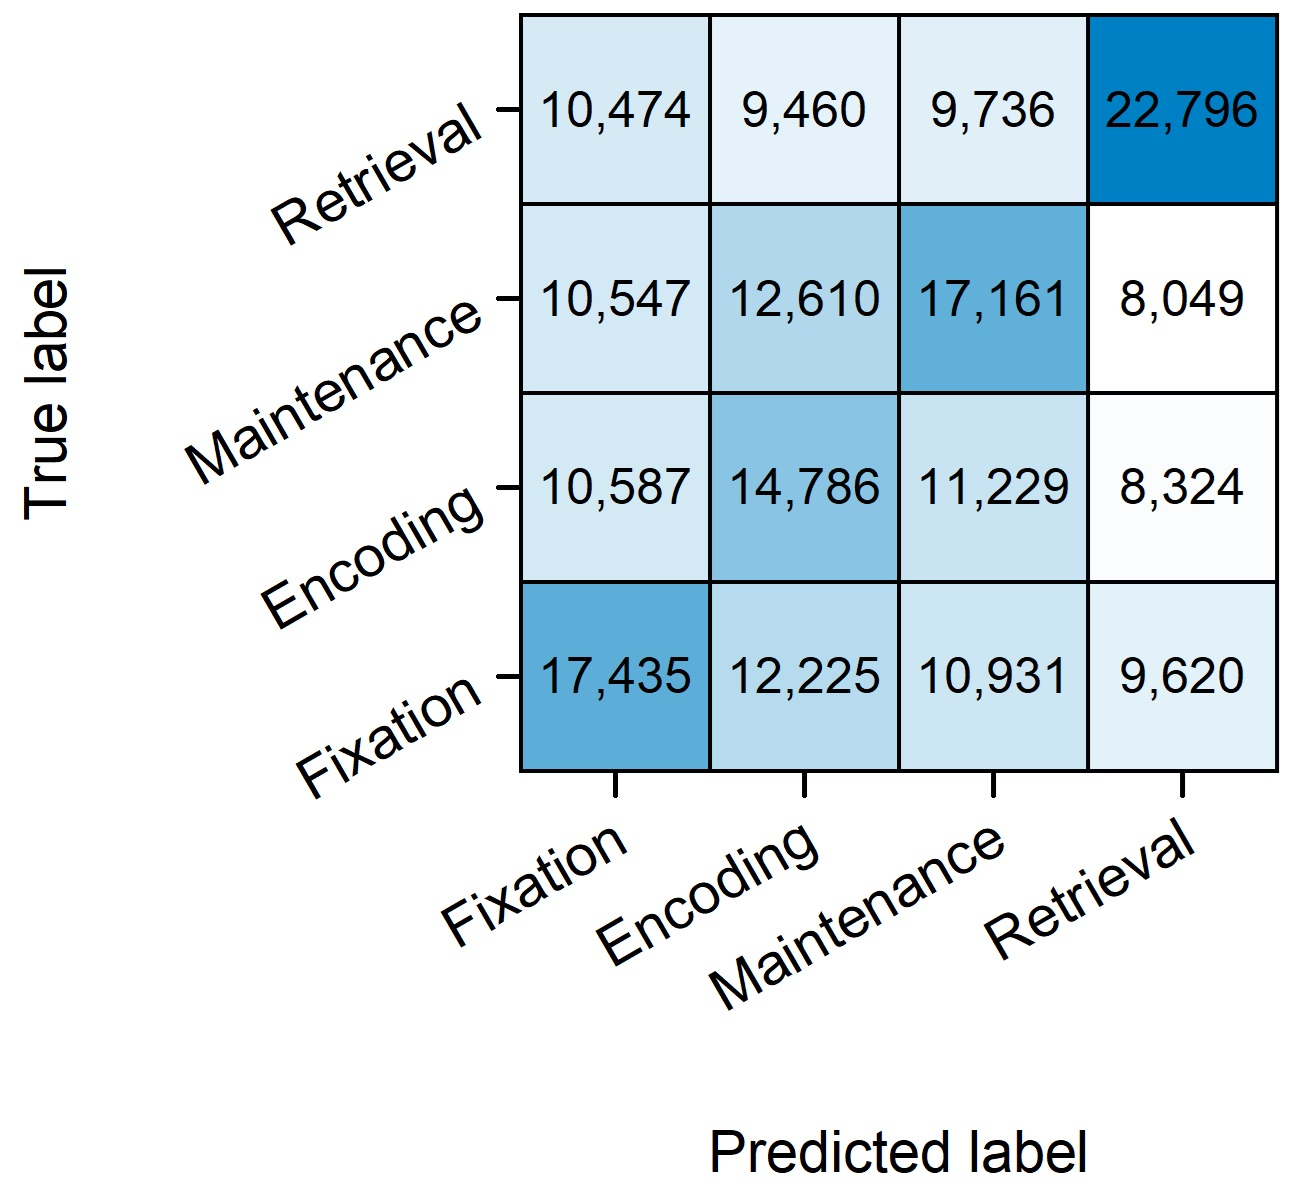
\includegraphics{./src/figures/LinearSVC/Figure_ID_SVC.jpg}

  % Table
  \begin{table*}[htbp]
    \centering
    \small
    \begin{tabular}{*{10}{c}}
      \toprule
      \textbf{\thead{}} &\textbf{\thead{cv_scores}} &\textbf{\thead{dummy_scores}} &\textbf{\thead{w_statistic}} &\textbf{\thead{p_value}} &\textbf{\thead{dof}} &\textbf{\thead{effsize}} &\textbf{\thead{sub}} &\textbf{\thead{session}} &\textbf{\thead{roi}} &\\
      \midrule
      0 & 0.411 +/- 0.111 & 0.246 +/- 0.092 & -14.313 & 0.0 & 185.417 & 0.137 & 01 & 01 & AHL\\
      \rowcolor{lightgray}
      1 & 0.383 +/- 0.109 & 0.253 +/- 0.099 & -10.034 & 0.0 & 197.633 & 0.197 & 01 & 02 & AHL\\
      2 & 0.381 +/- 0.101 & 0.232 +/- 0.091 & -13.838 & 0.0 & 181.167 & 0.143 & 03 & 01 & AHR\\
      \rowcolor{lightgray}
      3 & 0.428 +/- 0.106 & 0.244 +/- 0.103 & -17.52 & 0.0 & 192.872 & 0.109 & 03 & 02 & AHR\\
      4 & 0.407 +/- 0.093 & 0.264 +/- 0.104 & -12.735 & 0.0 & 178.127 & 0.152 & 04 & 01 & PHL\\
      \rowcolor{lightgray}
      5 & 0.486 +/- 0.105 & 0.252 +/- 0.091 & -32.141 & 0.0 & 197.049 & 0.053 & 04 & 02 & PHL\\
      6 & 0.346 +/- 0.090 & 0.259 +/- 0.095 & -7.152 & 0.0 & 197.016 & 0.257 & 06 & 01 & AHL\\
      \rowcolor{lightgray}
      7 & 0.329 +/- 0.086 & 0.239 +/- 0.090 & -7.963 & 0.0 & 194.355 & 0.238 & 06 & 02 & AHL\\
      8 & 0.507 +/- 0.108 & 0.254 +/- 0.100 & -38.482 & 0.0 & 197.153 & 0.041 & 09 & 01 & AHR\\
      \rowcolor{lightgray}
      9 & 0.490 +/- 0.098 & 0.265 +/- 0.091 & -34.298 & 0.0 & 186.034 & 0.046 & 09 & 02 & AHR\\
      10 & 0.417 +/- 0.117 & 0.251 +/- 0.096\\
      \bottomrule
    \end{tabular}
    \captionsetup{width=\textwidth}

    \caption{\textbf{
        SVC Classification of States
      }
      \smallskip
      \\
      SVC classification of NT states revealed linear distinguishability, confirming the existence of distinct states in NT spaces.
    }
    % width=1\textwidth

    \label{tab:04}
  \end{table*}
  \restoregeometry
  \DIFaddend
}
